\documentclass[11pt,a4paper]{article}
\usepackage[utf8]{inputenc}
\usepackage[spanish]{babel}
\usepackage{amsmath}
\usepackage{amsfonts}
\usepackage{amssymb}
\usepackage{makeidx}
\usepackage{graphicx}
\usepackage{lmodern}
\usepackage{kpfonts}
\usepackage{parskip}
\usepackage[left=2cm,right=2cm,top=2cm,bottom=2cm]{geometry}
\author{Miguel Angel Xamie Diaz Fuentes}
\begin{document}
\begin{center}
\begin{LARGE}
\textbf{INGENIERÍA MECATRÓNICA}\\
\end{LARGE}
{\large Sistemas Eletrónicos De Interfaz}\\
\begin{figure}[hbtp]
\centering

\includegraphics[scale=0.80]{UPZMG_Mecatr_nica.png}
\end{figure} 
\begin{center}
\begin{LARGE}
EV-2-7-DISEÑO DE UNA MODULACION DE ANCHO PULSO (PWM) CON AMP-OP Y TRANSISTORES
\end{LARGE}
\end{center}

\begin{Large}
\textbf{Alumno}
\\\textit{Miguel Angel Xamie Diaz Fuentes}
\textbf{\\Maestro}
\\\textit{Morán Garabito Carlos Enrique}
\textbf{\\Fecha de Entrega}
\\\textit{15/10/2019}
\textbf{\\Grupo}
\\\textit{4-B}\\
\textbf{Período Cuatrimestral}\\
\textit{2019-Septiembre-Diciembre}
\\
\end{Large}

\end{center}

\footnote{Universidad Politécnica De La Zona Metropolitana De Guadalajara} 

\newpage

\section{Introducción}

\begin{flushleft}
La modulación oir ancho de pulsos (también conocida como \textbf{PWM} de una señal o fuente de energía es una técnica en la que se modifica el ciclo de trabajo de una señal periódica (una senoidal o una cuadrada, por ejemplo), ya sea para transmitir información a través de un canal de comunicaciones o para controlar la cantidad de energía que se envía a una carga. EL cilo de trabajo de una señal periódica es el ancho relativo de su parte positiva en relación con el periódo. Expresado matemáticamente:\\
\end{flushleft}

{\huge $ \D = \frac{t}{T} $\\}\\
d = es el ciclo de trabajo\\
t = es el tiempo en que la función es positiva (ancho del pulso)\\
T = es el período de la función\\

\section{Diseño}

La construcción típica de un circuito PWM se lleva a cabo mediante un comparador con dos entradas y una salida. Una de las entradas se conecta a un oscilador de onda dientes de sierra, mientras que la otra queda disponible para la señal moduladora. En la salida la frecuencia es generalmente igual a la de la señal dientes de sierra y el ciclo de trabajo está en función de la portadora.\\

\begin{figure}[hbtp]
\centering
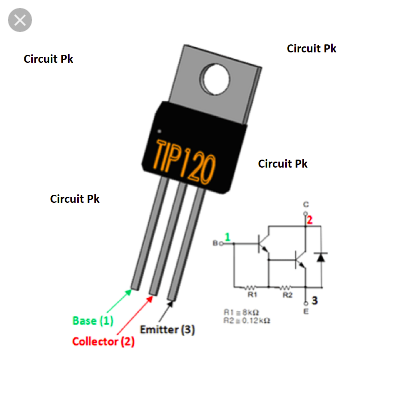
\includegraphics[scale=0.80]{1.png}
\end{figure} 

La principal desventaja que presentan los circuitos PWM es la posibilidad de que haya interferencias generadas por radiofrecuencia. EStas pueden minimizarse ubicando el controlador cerca de la carga y realizando un filtrado de la fuente de alimentación.


Hay muchas formas de generar este tipo de onda, utilizando compuertas, con un PIC, pero se usara el histórico 555, y aun con este hay varias formas de generarla, una de ellas es utilizando el tiempo de carga y descarga del condensador que controla los tiempos del 555, pero se utilizara la salida del 555 para cargar y descargar otro condensador por medio de un transistor.

\footnote{Universidad Politécnica De La Zona Metropolitana De Guadalajara} 

\newpage

\begin{figure}[hbtp]
\centering
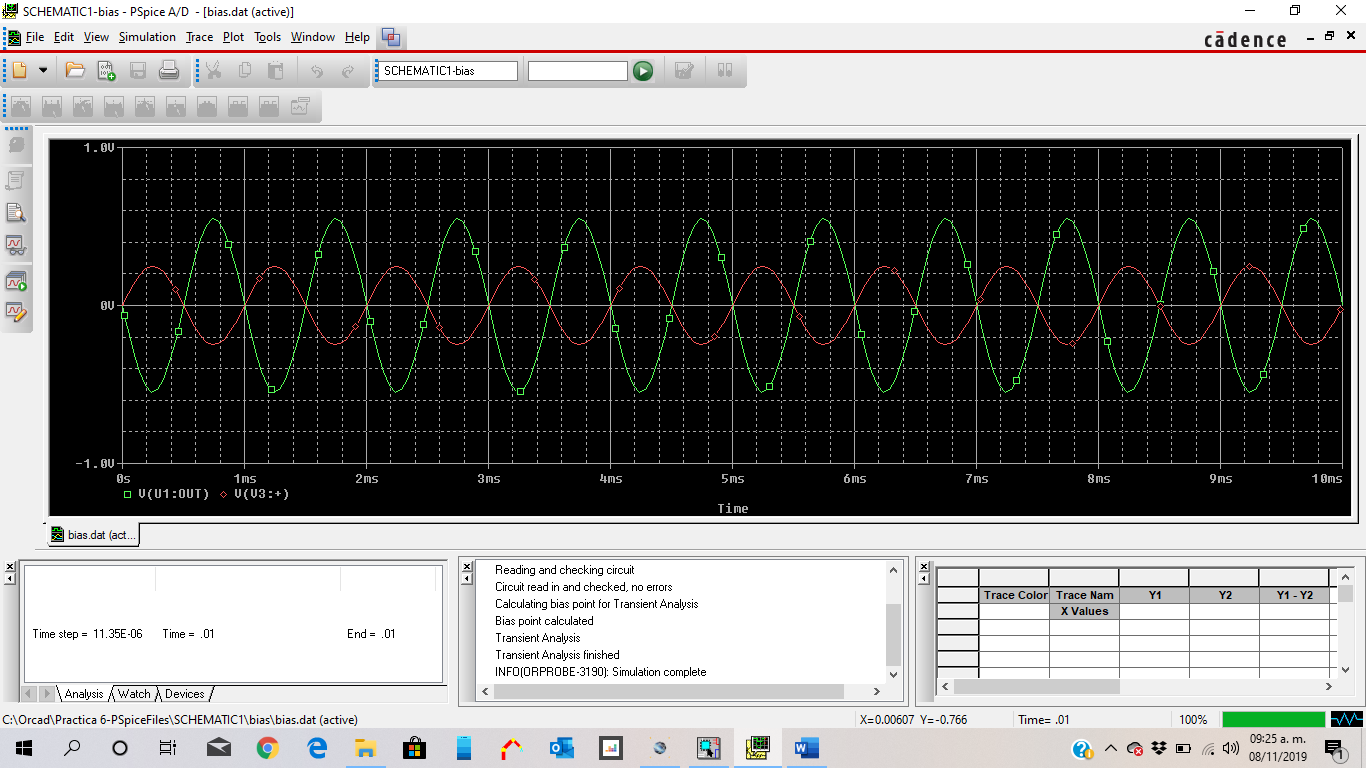
\includegraphics[scale=0.37]{2.png}
\end{figure} 

En este Diseño se compone de dos partes básicas, una el 555 configurado como estable con cierto periodo, donde el tiempo en alto es mayor al tiempo en bajo, tiempos que son invertidos gracias al inversor XD.
La segunda parte esta conformada por un condensador y un transistor, donde el transistor descarga por cada pulso al condensador generando así la onda con forma de dientes de sierra. 

\begin{figure}[hbtp]
\centering
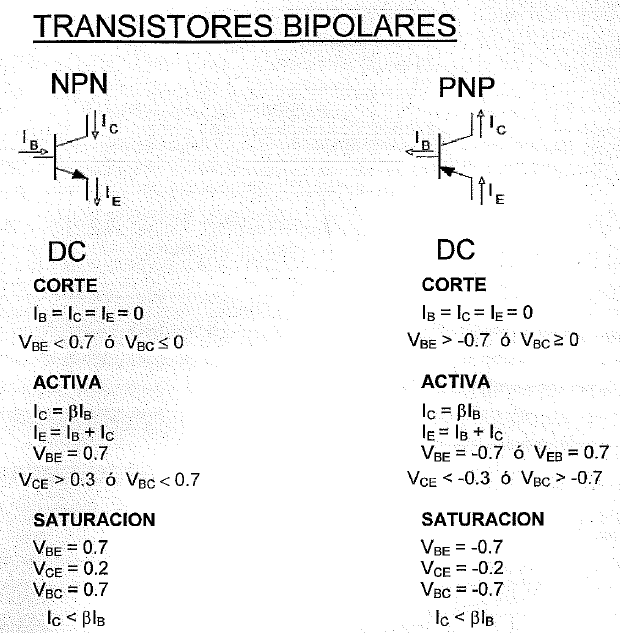
\includegraphics[scale=0.47]{3.png}
\end{figure} 

\textbf{Segundo}: Rampa (onda moduladora):

Es la parte mas sencilla de todo el diseño, se basa en el mismo concepto anterior de carga y descarga de un condensador, pero en este caso solo nos interesa la carga. 

\footnote{Universidad Politécnica De La Zona Metropolitana De Guadalajara} 

\newpage

\begin{figure}[hbtp]
\centering
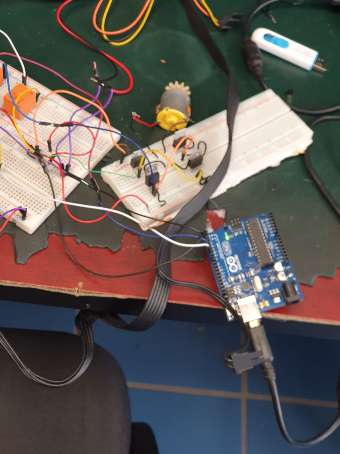
\includegraphics[scale=0.35]{4.png}
\end{figure} 

En este caso en vez de un transistor tenemos un switch, que por decirlo así es el encargado de poner en funcionamiento nuestro circuito, cuando esta cerrado el condensador esta descargado, no hay movimiento pero cuando se abre el condensador empieza a cargarse a determinada velocidad. 

\textbf{Tercero}: Integración de los dos circuitos:

Ya teniendo los circuitos medianamente claros XD, nos preguntamos ¿y bueno eso para que? pues bueno una circuito de PWM consta de dos tipos de onda, una portadora(triangular o dientes de sierra) y una moduladora (la rampa), que se comparan atravez de un amplificador operacional y generan la PWM. 

\begin{figure}[hbtp]
\centering
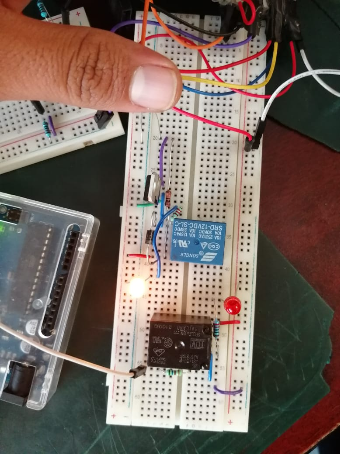
\includegraphics[scale=0.50]{6.png}
\end{figure} 

\footnote{Universidad Politécnica De La Zona Metropolitana De Guadalajara} 

\newpage

\textbf{Cuarto}: Carga:

Ya lo único que falta es la carga, es decir lo que quieres controlar con este medio, en este caso toco poner un motor. el mecanismo es fácil, solo se trata de un transistor, para mejor uso un MOSFET, y la carga, el gate del MOSFET va conectada a la salida del amplificador operacional, el drain y el source son ya parte del otro circuito (a controlar).

\begin{figure}[hbtp]
\centering
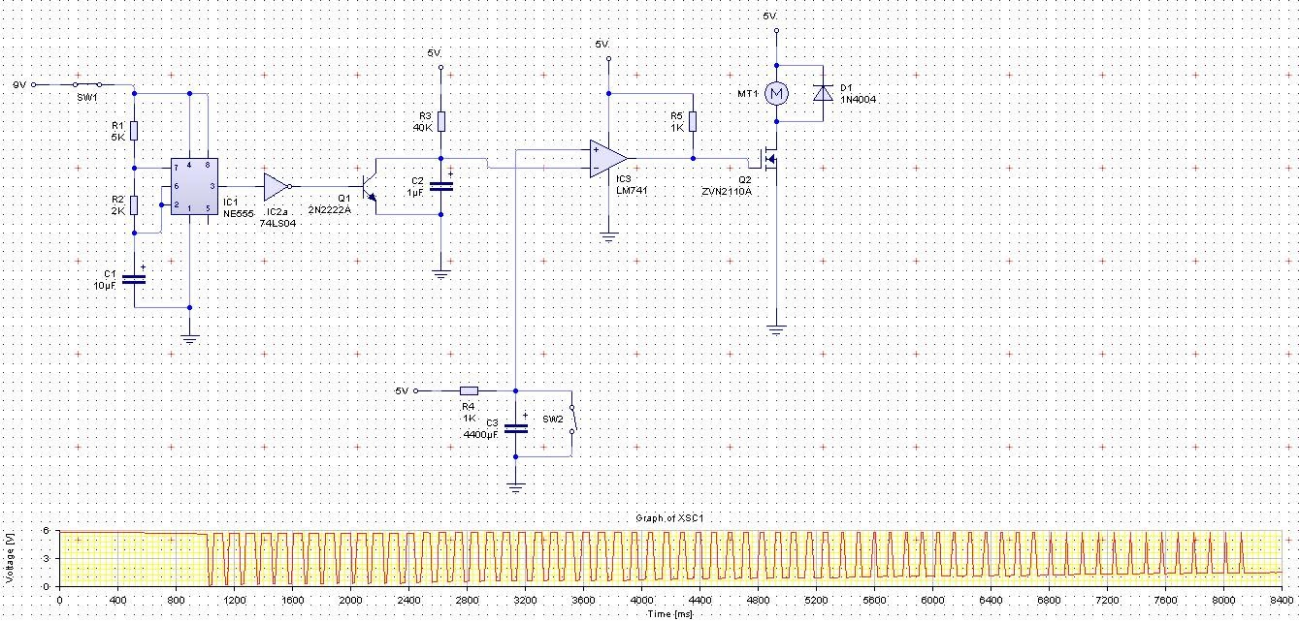
\includegraphics[scale=0.35]{5.png}
\end{figure} 

Como dato el \textbf{Integrado 555} Fue introducido primero por la Signetics Corporation, y  es similar a los amplificadores operacionales de propósito general, porque el 555 es confiable, fácil de usar y de bajo costo.
Se puede usar para operar con voltajes entre +5v a +18v, por lo tanto sirve con circuitos TTL (lógica de transistor - transistor), como con amplificadores operacionales. Se encuentra en aplicaciones como: osciladores, generadores de pulso, generadores de rampa u onda cuadrada, multivibrador de disparo, alarmas contra robo y monitor,

\begin{figure}[hbtp]
\centering
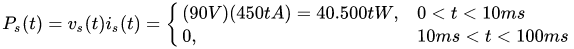
\includegraphics[scale=0.70]{7.png}
\end{figure} 

\footnote{Universidad Politécnica De La Zona Metropolitana De Guadalajara} 

\newpage



\section{Aplicaciones}

En la actualidad existen muchos circuitos integrados en los que se implementa la modulación PWM, además de otros muy particulares para lograr circuitos funcionales que puedan controlar fuentes conmutadas, controles de motores, controles de elementos termoeléctricos, choppers para sensores en ambientes ruidosos y algunas otras aplicaciones. Se distinguen por fabricar este tipo de integrados compañías como Texas Instruments, National Semiconductor, Maxim, y algunas otras más. 

\subsection{Información sobre PWM}
\textbf{Pérdidas de energía en un regulador de conmutación de voltaje}

La técnica más común para regular el voltaje de un dispositivo de conmutación es utilizar un oscilador y controlador de PWM para producir una onda de pulso rectangular que alterna la unidad interna del MOSFET (o de los MOSFET en un dispositivo sincrónico) a una frecuencia establecida generalmente en un rango de cientos de megahercios. (Las frecuencias más altas permiten componentes magnéticos más pequeños a expensas de los desafíos de una mayor interferencia electromagnética (EMI].) El voltaje de salida del regulador es proporcional al ciclo de trabajo de la onda PWM.

En general, la técnica funciona bien, pero en cargas bajas se compromete la eficiencia. Para comprender el motivo, resulta beneficioso considerar dónde ocurren las pérdidas de energía, ya que la energía que se extrae en la entrada del regulador de voltaje no se transfiere a la carga de salida. 


\bibliography{Referencia}
\begin{thebibliography}{X}
\bibitem{Baz} \textsc{THE DECCA DIGITAL.} \textit{Electrónica de  potencia.}Multiplexación.

\bibitem{Baz} \textsc{MANCINI, GINO.} \textit{Modulación por impulsos codificados.} 
Mastering System (2007).


\bibitem{Baz} \textsc{JUAN MANZANO ULMEHER.} \textit{Digital singnaling techniques.} 
Communications Megazine (IEEE).
\bibitem{Baz} \textsc{RONALD J. TOCCI, NEAL S. WID,ER, GREGPRY L. MOSS.} \textit{Sistemas digitales: comienzos y aplicaciones.} 
Pearson Educación. ISBN(1205524427, 47852114512).

\end{thebibliography}

\bibliographystyle{plain}




\footnote{Universidad Politécnica De La Zona Metropolitana De Guadalajara} 




\end{document}